% ======================================================================
% Chapter 1: Data basics (SAMPLE questions for the guide)
% Group: ch01_data      ID prefix: DATA
% One question per \element. Every \element in this file uses the same group.
% ======================================================================

\element{ch01_data}{
\begin{question}{DATA001}
A shop records each customer's postcode. On which scale of measurement is a postcode?
\begin{choices}
  \correctchoice{Nominal}
  \wrongchoice{Ordinal}
  \wrongchoice{Interval}
  \wrongchoice{Ratio}
\end{choices}
\explain{A postcode is a label: it has no order and arithmetic on it means nothing.}
\end{question}
}

\element{ch01_data}{
\begin{question}{DATA002}
A survey asks customers to rate a service as poor, fair, good or excellent. On which scale is the answer?
\begin{choices}
  \wrongchoice{Nominal}
  \correctchoice{Ordinal}
  \wrongchoice{Interval}
  \wrongchoice{Ratio}
\end{choices}
\end{question}
}

\element{ch01_data}{
\begin{question}{DATA003}
Which of these is unstructured data?
\begin{choices}
  \wrongchoice{A table of daily sales}
  \wrongchoice{A list of product prices}
  \correctchoice{Recorded customer phone calls}
  \wrongchoice{A spreadsheet of staff IDs}
\end{choices}
\end{question}
}

\element{ch01_data}{
\begin{question}{DATA004}
The table shows four orders. Which column has a missing value?

\begin{center}
{\small
\begin{tabular}{|c|c|c|}
\hline
Order & Item & Price \\ \hline
101 & Pen & 20 \\
102 & Book & \\
103 & Bag & 450 \\
104 & Cup & 60 \\ \hline
\end{tabular}}
\end{center}
\begin{choices}
  \wrongchoice{Order}
  \wrongchoice{Item}
  \correctchoice{Price}
  \wrongchoice{None of the columns}
\end{choices}
\end{question}
}

\element{ch01_data}{
\begin{question}{DATA005}
The chart shows monthly sales. In which month were sales highest?

\begin{center}
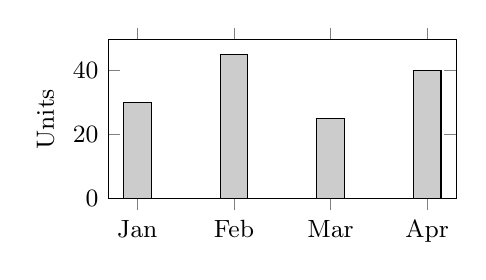
\begin{tikzpicture}
\begin{axis}[ybar, width=6cm, height=3.6cm, bar width=10pt,
             symbolic x coords={Jan,Feb,Mar,Apr}, xtick=data,
             ymin=0, ylabel={Units}, ylabel style={font=\small},
             tick label style={font=\small}]
\addplot[fill=gray!40] coordinates {(Jan,30) (Feb,45) (Mar,25) (Apr,40)};
\end{axis}
\end{tikzpicture}
\end{center}
\begin{choices}
  \wrongchoice{January}
  \correctchoice{February}
  \wrongchoice{March}
  \wrongchoice{April}
\end{choices}
\end{question}
}

\element{ch01_data}{
\begin{question}{DATA006}
A temperature sensor sends a reading every second. Which characteristic of big data does this describe?
\begin{choices}
  \wrongchoice{Volume}
  \correctchoice{Velocity}
  \wrongchoice{Variety}
  \wrongchoice{Veracity}
\end{choices}
\end{question}
}

\element{ch01_data}{
\begin{question}{DATA007}
Many customer addresses in a database are misspelled or duplicated. Which characteristic of big data is the problem?
\begin{choices}
  \wrongchoice{Volume}
  \wrongchoice{Velocity}
  \wrongchoice{Variety}
  \correctchoice{Veracity}
\end{choices}
\end{question}
}

\element{ch01_data}{
\begin{question}{DATA008}
A bank stores customer records in tables with fixed columns. What kind of data is this?
\begin{choices}
  \correctchoice{Structured data}
  \wrongchoice{Unstructured data}
  \wrongchoice{Streaming data}
  \wrongchoice{Image data}
\end{choices}
\end{question}
}
